Цель данной работы "--- написать программу с графическим пользовательским интерфейсом, предоставляющую определённые средства для разработки задач по олимпиадному программированию и для тестирования решений к созданным задачам. Рассмотрим основные варианты использования, которые необходимо реализовать. Так как разработку задач и тестирование решений можно рассматривать отдельно, варианты использования изображены ниже на двух отдельных диаграммах.

На рис.~\ref{use_case_diagram_development} изображена диаграмма вариантов использования, связанных с разработкой задач. Предполагается возможность прикреплять к задаче определённые параметры (такие, как ограничения по времени и памяти, условие задачи), а также "--- тесты, генераторы, валидаторы, чекеры и авторские решения (подробнее обо всём этом речь пойдёт в следующей главе).

\begin{figure}[!b]
\center{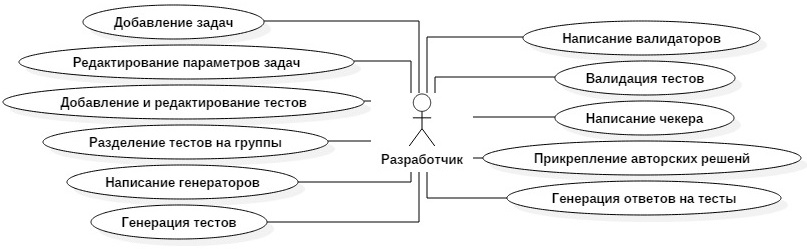
\includegraphics[scale=0.85]{use_case_diagram_development}}
\caption{Варианты использования (разработка задач)}
\label{use_case_diagram_development}
\end{figure}

Создаваемое приложение должно давать возможность писать код для генераторов, валидаторов и чекеров прямо в своём графическом интерфейсе. Это предполагает также написание специальной библиотеки для разработки задач. Эта библиотека будет предоставлять методы с реализацией типичных операций, и пользователь сможет вызывать их прямо из своего кода. Кроме того, все перечисленные средства разработки можно будет компилировать и запускать из самого приложения.

Диаграмма на рис.~\ref{use_case_diagram_testing} отражает варианты использования, связанные с тестированием решений. Заметим здесь, что предполагается возможность отправлять решения, написанные на разных языках: в данной работе мы реализуем поддержу всего двух языков программирования "--- Java и C++. Также приложение должно будет поддерживать различные системы оценивания (их мы также подробно рассмотрим в следующей главе).

\begin{figure}[h]
\center{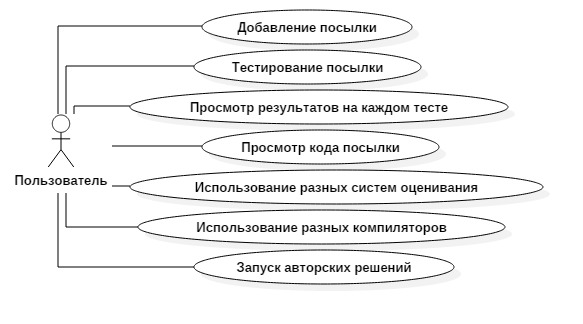
\includegraphics[scale=0.7]{use_case_diagram_testing}}
\caption{Варианты использования (тестирование)}
\label{use_case_diagram_testing}
\end{figure}

Приложение будет сохранять всю информацию в файловой системе и не будет использовать никаких баз данных. По определённому пути, который пользователь сможет выбрать, будет находиться определённая иерархия папок, в которых будут храниться все создаваемые и отправляемые файлы: условия задач, тесты, генераторы, валидаторы, чекеры, авторские и прочие решения, конфигурационные файлы. Все параметры, которые будут прикрепляться к задачам и решениям, будут также храниться в файловой системе в XML-дескрипторах.